\documentclass[8pt]{article}

\usepackage[margin=1in]{geometry}
\usepackage{amsmath,amssymb}
\usepackage{wrapfig}
\usepackage{multicol}
\usepackage{graphicx}
\usepackage{makecell}

\graphicspath{{figs/}}
\newcommand{\sect}[1]{\noindent\textbf{#1}\\}
\newcommand{\hl}{\noindent\makebox[\linewidth]{\rule{\textwidth}{0.2pt}}}
\newcommand\tab[1][1cm]{\hspace*{#1}}

\begin{document}
	\noindent\begin{center}\textbf{Equations for Exam \#3}\end{center}
	\setlength{\columnseprule}{0.4pt}
	\begin{multicols*}{2}
		\begin{small}
		\sect{General:}
		$\phi_F = \cfrac{kT}{q} \text{ln} \cfrac{N_a}{n_i}$ \\
		$ V_T = V_P - V_0 $, \tab[0.25cm] $ V_0 = \cfrac{kT}{q} \ln \cfrac{N_a N_d}{n_i^2} $ \\
		\sect{JFETs:}
		$ V_P = \cfrac{q a^2 N_d}{2\varepsilon} $ \\
		$ |V_D(\text{sat.})| = |V_P| - |V_{GS}| - |V_0| $ \\
		$ I_D = G_0V_P\left[ \cfrac{V_D}{V_P} + \frac{2}{3}\left( -\cfrac{V_G}{V_P} \right)^{\frac{3}{2}} - \frac{2}{3} \left( \cfrac{V_D-V_G}{V_P} \right)^{\frac{3}{2}} \right] $ \\
		$ I_D(\text{sat.}) = G_0V_P\left[ \cfrac{V_D}{V_P} + \frac{2}{3} \left( - \cfrac{V_G}{V_P} \right)^{3/2} - \frac{2}{3} \right]  $ \\
		\tab[1.21cm] $ = G_0 V_P \left[ \cfrac{V_G}{V_P} + \frac{2}{3} \left( - \cfrac{V_G}{V_P} \right)^{3/2} + \frac{1}{3} \right] $ \\
		$ \cfrac{V_D}{V_P} = 1 + \cfrac{V_G}{V_P} $ \\
		$ G_0 = 2aq\mu_nn\cfrac{Z}{L} $ \\
		$ g_m(\text{sat.}) = G_0 \left[ 1 - \left(-\cfrac{V_G}{V_P}\right)^{1/2} \right] $\\
		\sect{Metal-Semiconductor FET:}
		$v_d = \cfrac{\mu \mathcal{E}}{1 + \mu \mathcal{E} / v_s} $ \\
		$ I_D = qnv_sA=qN_dv_sZh $ \\
		\sect{Metal-Insulator-Semiconductor FET:}
		$\phi_s(\text{inverted}) = 2\phi_F = 2\cfrac{kT}{q} \ln \cfrac{N_a}{n_i} $ \\
		$ L_D = \sqrt{\cfrac{\epsilon_s k T}{q^2 p_0}} $ \\
		$ V_i = \cfrac{-Q_s}{C_i} $ \\
		$ W = \left[ \cfrac{2 \varepsilon_s \phi_s}{qN_a} \right]^{1/2} $\\ 
		$ W_m = 2 \left[ \cfrac{\epsilon_s \phi_F}{q^2 N_a} \right]^{1/2} $ \\
		$ Q_d = -qN_aW_m = -2(\epsilon_sqN_a\phi_F)^{1/2} $ \\
		$ C_i = \cfrac{\varepsilon_i}{d} $, \tab[0.25cm] $ C_d = \cfrac{\epsilon_s}{W} $ \\
		$ C_{min} = \cfrac{C_iC_d}{C_i + C_d} $ \\
		$ V_{FB} = \Phi_{ms} - \cfrac{Q_i}{C_i} $ \\
		$ V_T = -\cfrac{Q_d}{C_i} + 2\phi_F = V_{FB} - \cfrac{Q_d}{C_i} + 2h_f $ \\
		\tab[0.4cm] $ = \Phi_{ms} - \cfrac{Q_i}{C_i} - \cfrac{Q_d}{C_i} + 2\phi_F $ \\
		\begin{tabular}{l|c|c|c|c}
			$V_T = $ & $ \Phi_{ms} $ & $ -\cfrac{Q_i}{C_i} $ & $ -\cfrac{Q_d}{C_i} $ & $ + 2\phi_F$ \\ 
			& (-) & (-) & \makecell{(+) n channel \\ (-) p channel} & \makecell{(+) n channel \\ (-) p channel}
		\end{tabular}
		$ V_D(\text{sat.}) \approx V_G - V_T $ \\
		$ C_{debye} = \cfrac{\varepsilon_s}{L_D} $ \\
		$ D_{it} = \frac{1}{q} \left( \cfrac{C_iC_{LF}}{Ci - C_{LF}} - \cfrac{C_iC_{HF}}{C_i - C_{HF}} \right) \text{cm}^{-2} \text{eV}^{-1} $ \\
		\sect{MOSFET:}
		$ Q_s = Q_n + Q_d$ \\
		$ Q_n = -C_i \left[ V_G - \left( V_{FB} + \phi_s - \cfrac{Q_d}{C_i} \right)\right] $ \\
		$ V_G = V_{FB} - \cfrac{Q_s}{C_i} + \phi_s $ \\
		$ V_D(\text{sat.}) = |V_G| - |V_T| $ \\
		$ I_D = \cfrac{\overline{\mu_n} Z C_i}{L} \left[ \left( V_G - V_T \right) V_D - \frac{1}{2} V_D^2 \right] $ \\
		$ g = g_m(\text{sat.}) \approx \cfrac{Z}{L} \overline{\mu_n}C_i\left( V_G - V_T \right) $ \\
		$ I_D(\text{sat.}) \approx \frac{1}{2} \overline{\mu_n} C_i \cfrac{Z}{L} \left( V_G - V_T \right)^2 = \cfrac{Z}{2L} \overline{\mu_n}C_iV_D^2(\text{sat.}) $ \\
		$ I_D = \cfrac{\overline{\mu_n} Z C_i}{L \{1 + \theta(V_G - V_T) \}} \left[ (V_G - V_T)V_D - \frac{1}{2} V_D^2 \right] $ \\~\\~\\
		$\begin{aligned}
		I_D = \cfrac{\overline{\mu_n} Z C_i }{L} \left\{ (V_G - V_{FB} - 2\phi_F - \frac{1}{2}V_D)V_D \right. \\
		 \left. - \frac{2}{3} \cfrac{\sqrt{2\epsilon_sqN_a}}{C_i}[(V_D + 2\phi_F)^{3/2} - (2\phi_F)^{3/2}] \right\}
		\end{aligned}$\\~\\~\\
		\tab[0.53cm] $v = \mu \mathcal{E} \text{ for } \mathcal{E} < \mathcal{E}_{sat}$ \\
		and $ v = v_s \text{ for } \mathcal{E} > \mathcal{E}_{sat} $ \\
		\sect{Short Channel Characteristics:}
		$ I_D(\text{sat.}) \approx ZC_i(V_G - V_T)v_s $ \\
		\tab[1.23cm] $ \approx \left\{\cfrac{1 - r}{1 + r}\right\} ZC_i(V_G-V_T)v_{inj} $ \\
		\sect{Subthreshold Characteristics:}
		$ I_D = \mu(C_d + C_{it}) \cfrac{Z}{L}\left( \cfrac{kT}{q} \right)^2\left( 1 - e^{\frac{-qV_n}{kT}} \right) \left( e^{\frac{q(V_G-V_T)}{c_rkT}} \right) $ \\
		$ c_r = \left[ 1 + \cfrac{C_d + C_{it}}{C_i} \right] $ \\
		\sect{Drain Induced Barrier Lowering:}
		$ I_D = \cfrac{Z}{2L} \overline{\mu_n} C_i \left( V_G - V_T \right)^2 \left( 1 + \lambda V_D \right) $\\~\\
		\sect{Constants:}
		$q = 1.6\times10^{-19}$C\\
		$\epsilon_0 = 8.85\times10^{-14}$ Fm$^{-1}$,  $\epsilon_{r_{Si}} = 11.8$\\
		$ \epsilon_r(\text{SiO}_2) = 3.9 $ \\
		$h = 6.626 \times 10^{-34}$ m$^2$kg/s, \tab[0.25cm] $\hbar = 1.055 \times 10^{-31} $ Js/rad\\ 
		$m^* = 9.11 \times 10^{-31}$ kg\\
		$kT|_{T=300K} \approx 0.026$ eV \\
		$n_i(Si)|_{300K} = 1.5 \times 10^{10}$ cm$^{-3}$\\
		$v_{th} =$ Thermal Velocity $\approx 10^7$ cm/sec \\
		$\vec{\varepsilon}_c =$ critical field $= 10^4$ V/cm
		\end{small}
	\end{multicols*}
	
	\begin{center}
		\sect{\Large{Old Figures}}
		\includegraphics[width=\textwidth]{fig1} \\ \hl \\~\\
		\includegraphics[width=\textwidth]{fig2} \\ \hl \\~\\
		\includegraphics[width=\textwidth]{fig3} \\ \hl \\~\\
		\sect{\Large{Transistor Operation}}
		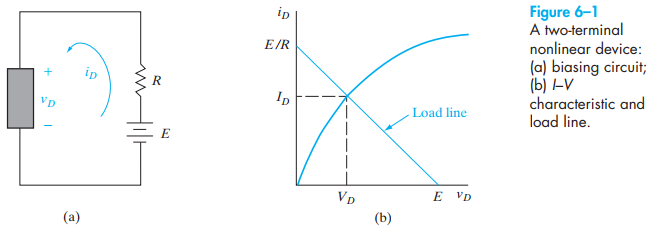
\includegraphics[width=0.7\textwidth]{fig6-1} \\ \hl \\~\\
		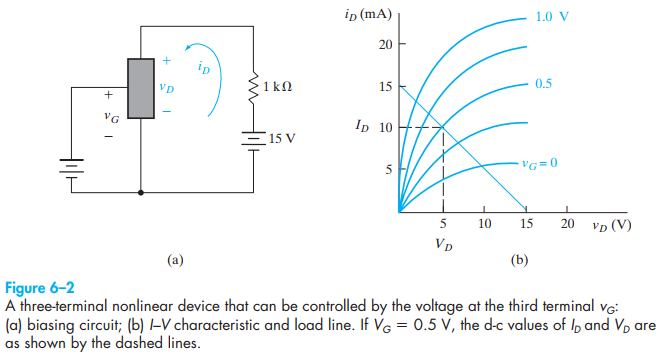
\includegraphics[width=0.7\textwidth]{fig6-2} \\ \hl \\~\\
		\sect{\Large{The Junction FET}}
		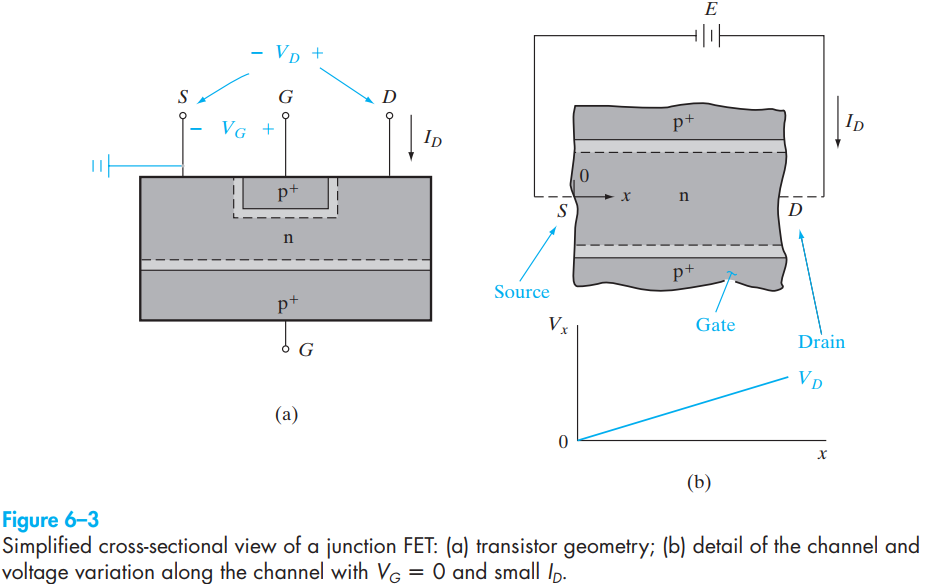
\includegraphics[width=0.7\textwidth]{fig6-3} \\ \hl \\~\\
		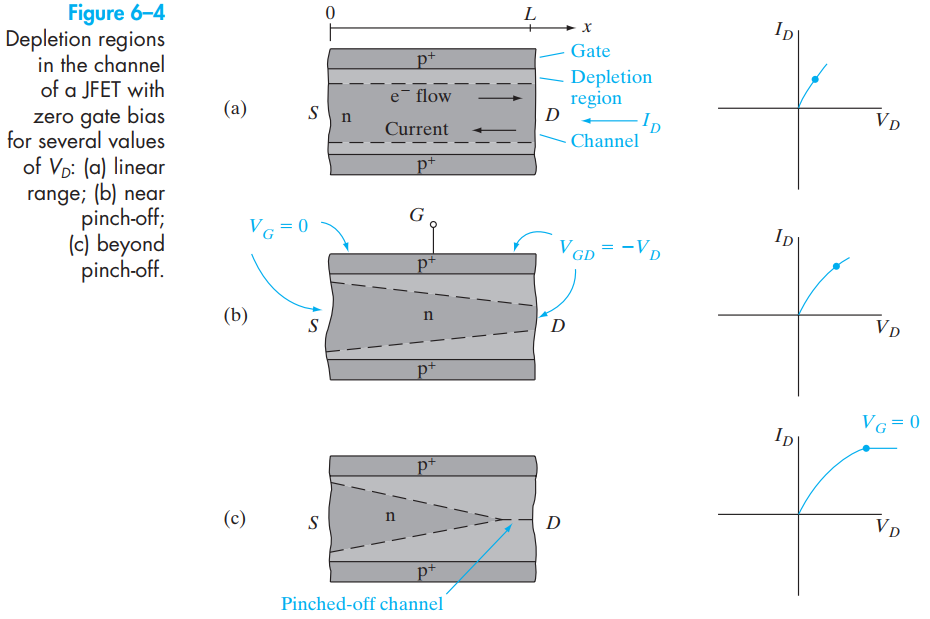
\includegraphics[width=0.7\textwidth]{fig6-4} \\ \hl \\~\\
		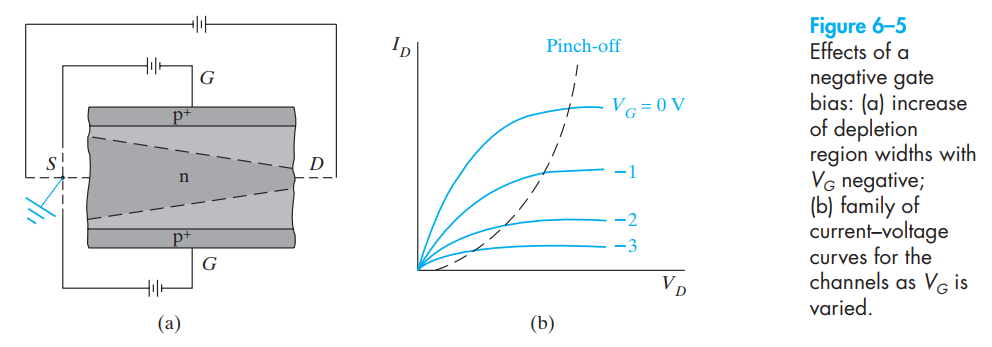
\includegraphics[width=0.7\textwidth]{fig6-5} \\ \hl \\~\\
		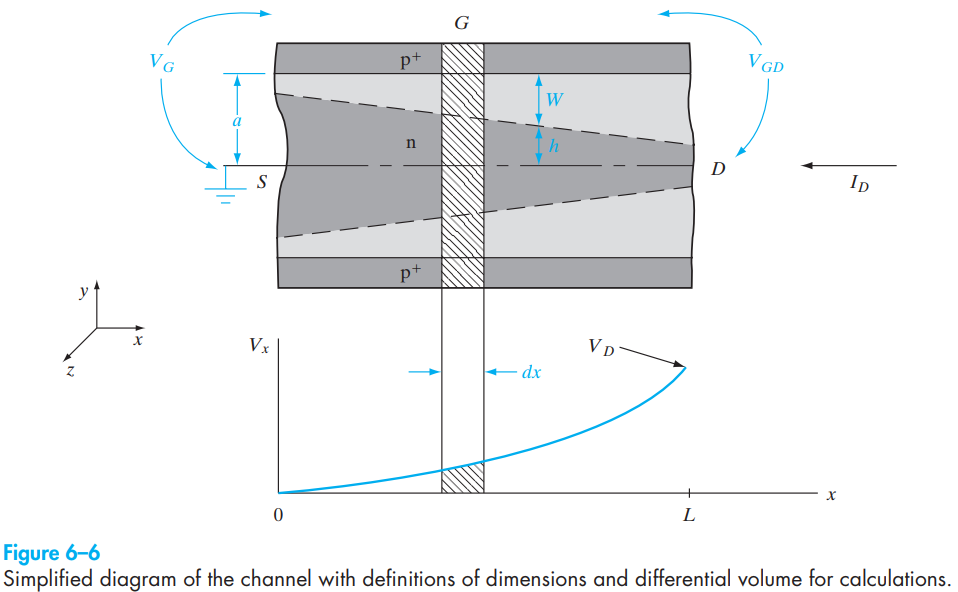
\includegraphics[width=0.7\textwidth]{fig6-6} \\ \hl \\~\\
		\sect{\Large{The Metal-Semiconductor FET}}
		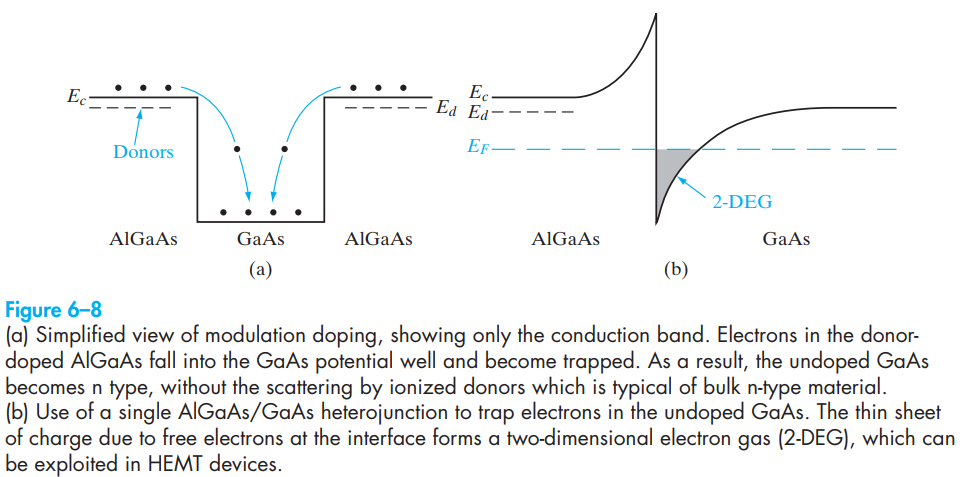
\includegraphics[width=0.7\textwidth]{fig6-8} \\ \hl \\~\\
		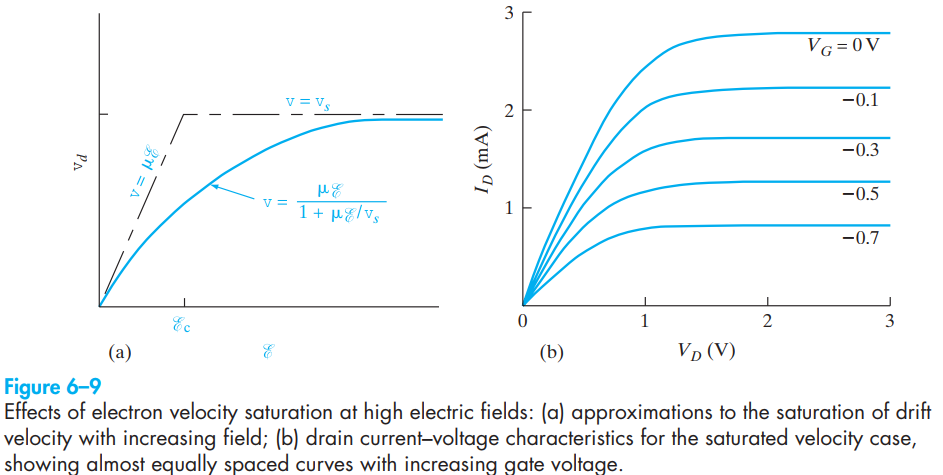
\includegraphics[width=0.7\textwidth]{fig6-9} \\ \hl \\~\\
		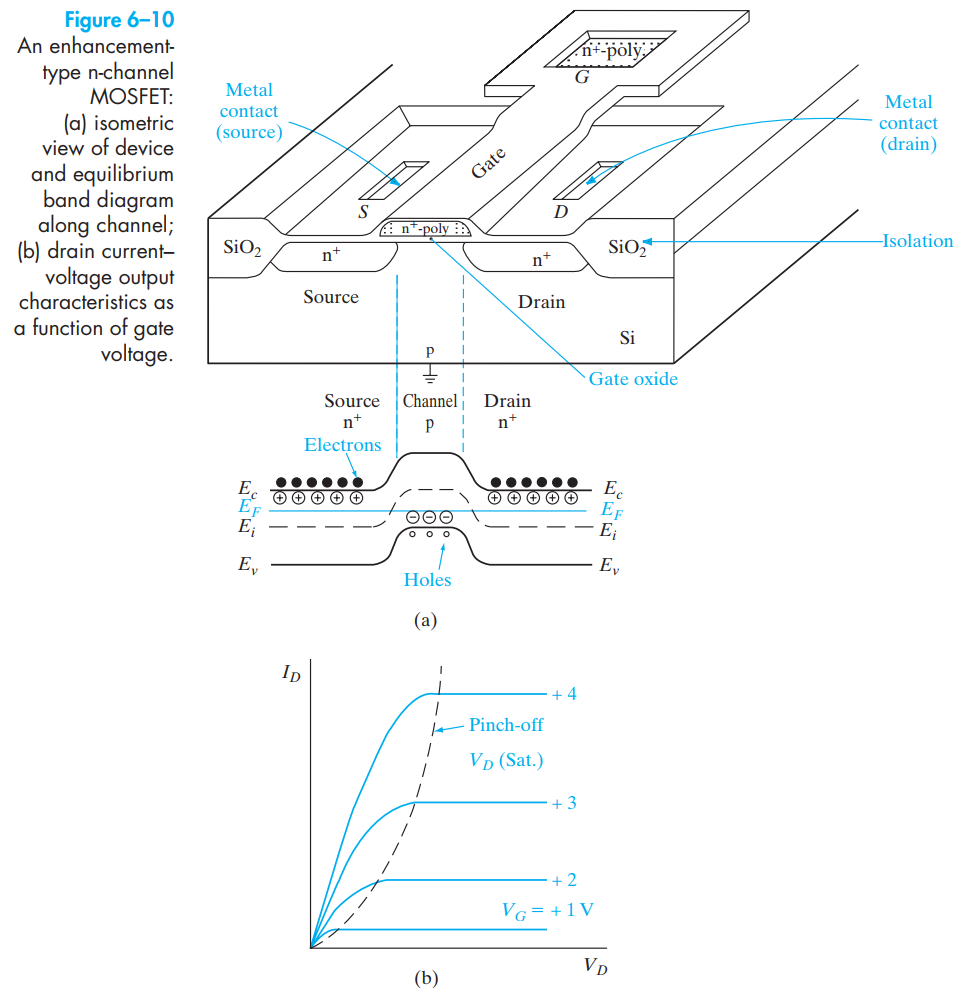
\includegraphics[width=0.7\textwidth]{fig6-10} \\ \hl \\~\\
		\sect{\Large{The Metal-Insulator-Semiconductor FET}}
		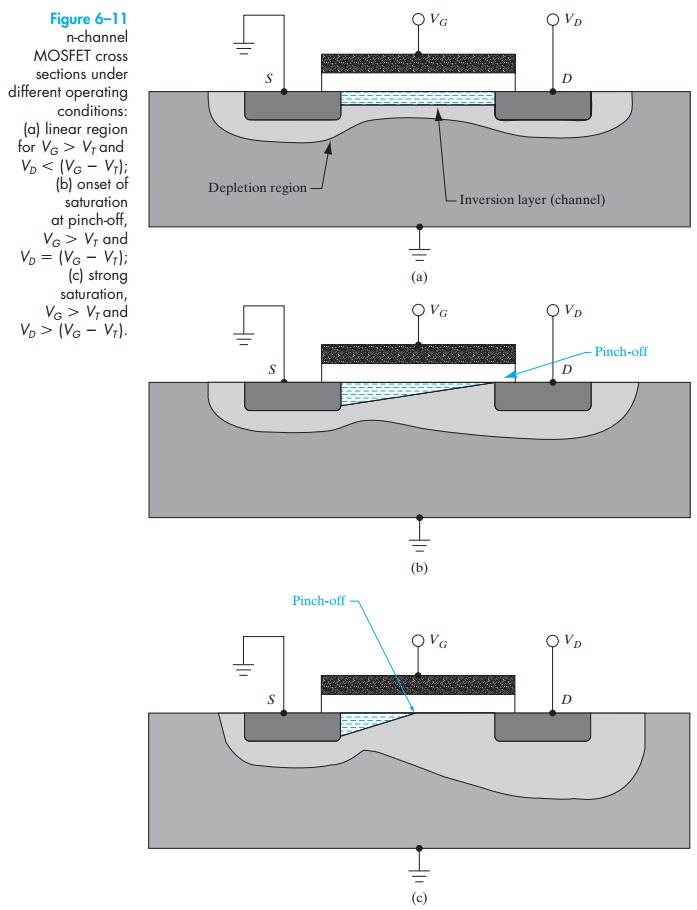
\includegraphics[width=0.7\textwidth]{fig6-11} \\ \hl \\~\\
		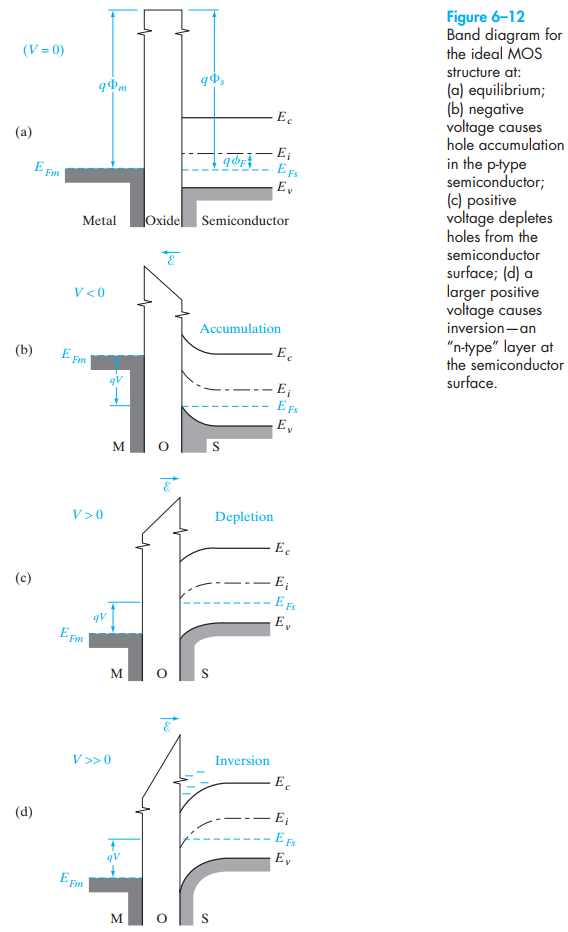
\includegraphics[width=0.7\textwidth]{fig6-12} \\ \hl \\~\\
		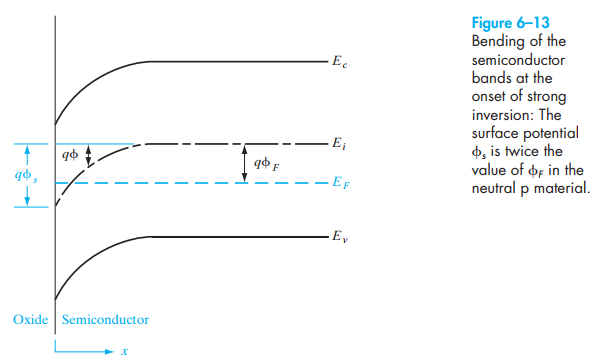
\includegraphics[width=0.7\textwidth]{fig6-13} \\ \hl \\~\\
		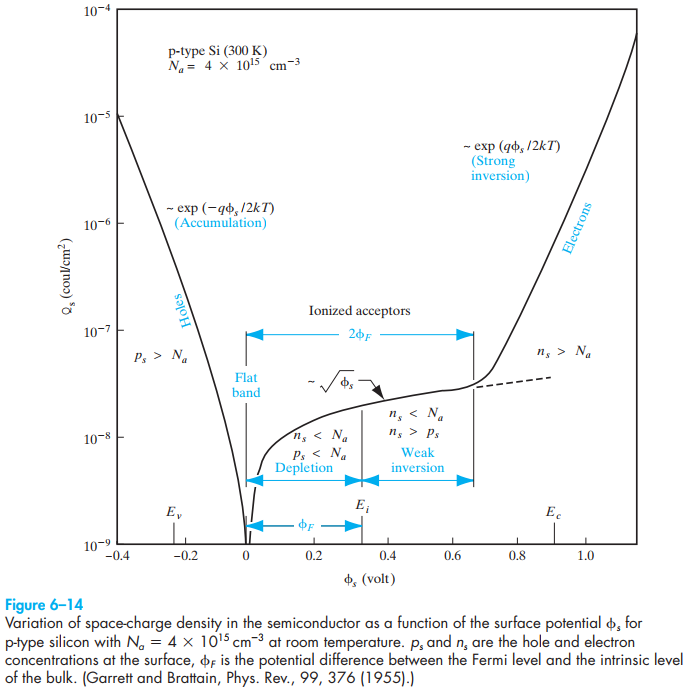
\includegraphics[width=0.7\textwidth]{fig6-14} \\ \hl \\~\\
		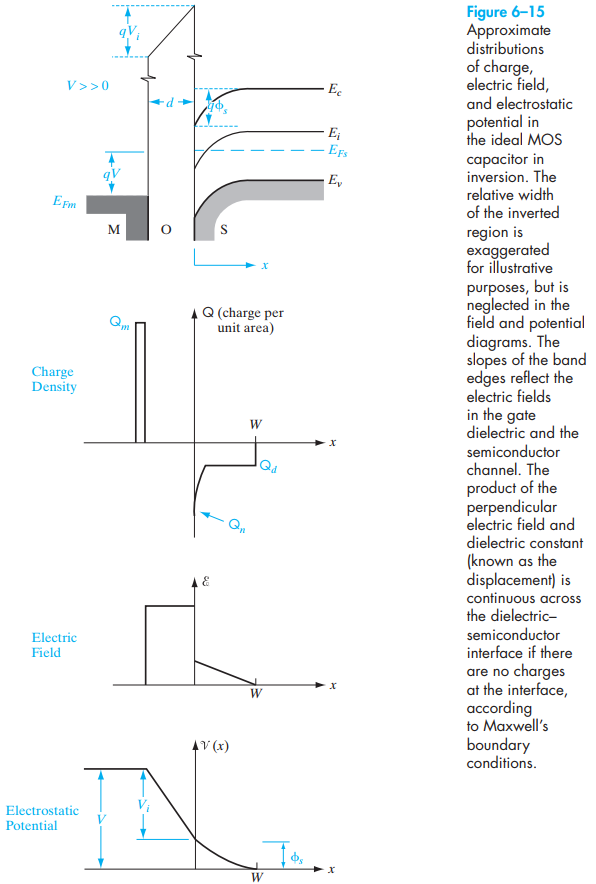
\includegraphics[width=0.7\textwidth]{fig6-15} \\ \hl \\~\\
		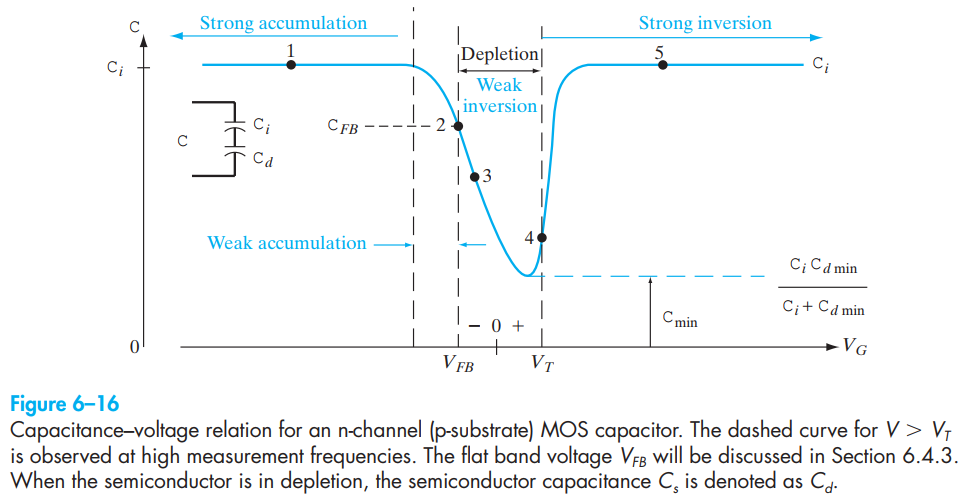
\includegraphics[width=0.7\textwidth]{fig6-16} \\ \hl \\~\\
		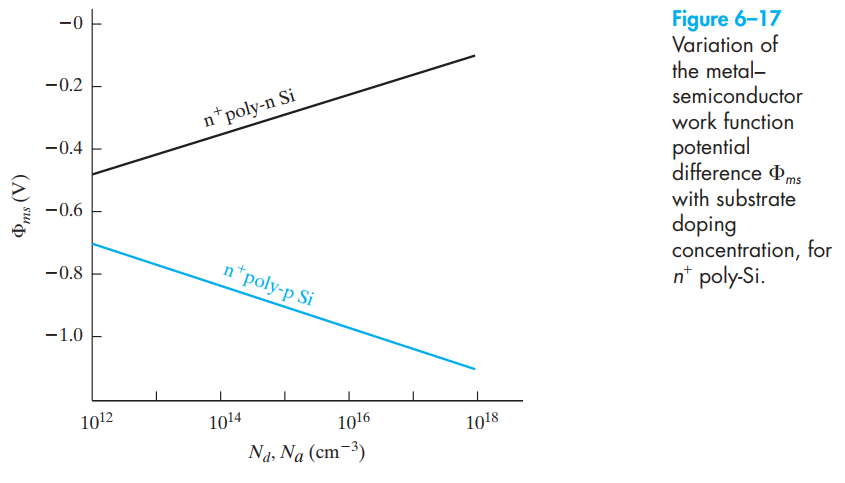
\includegraphics[width=0.7\textwidth]{fig6-17} \\ \hl \\~\\
		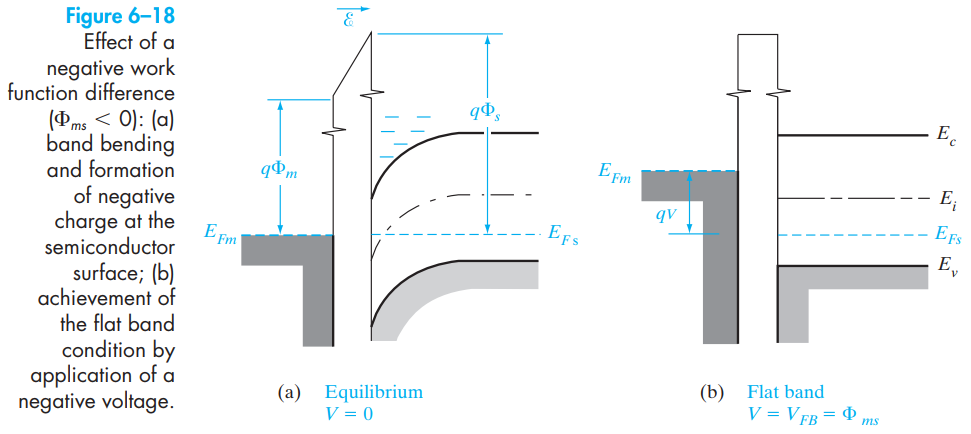
\includegraphics[width=0.7\textwidth]{fig6-18} \\ \hl \\~\\
		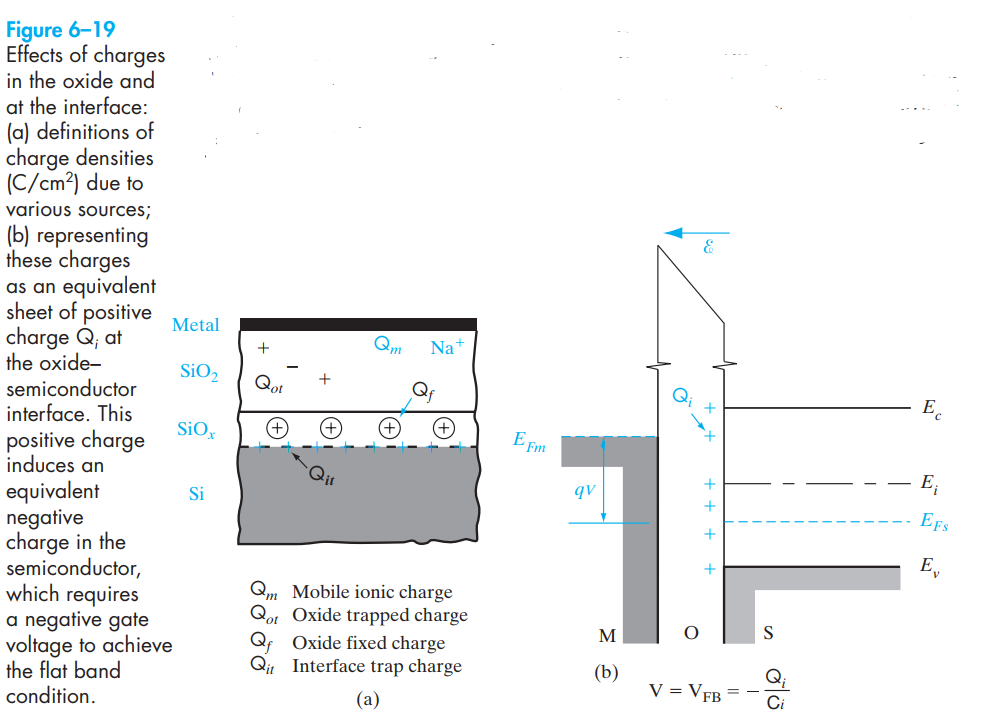
\includegraphics[width=0.7\textwidth]{fig6-19} \\ \hl \\~\\
		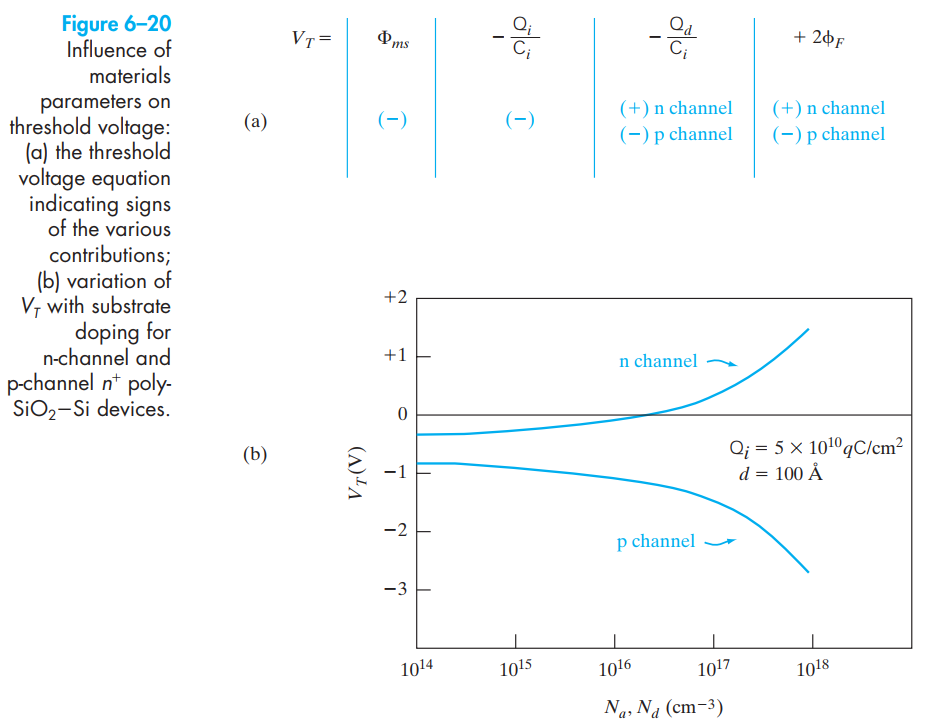
\includegraphics[width=0.7\textwidth]{fig6-20} \\ \hl \\~\\
		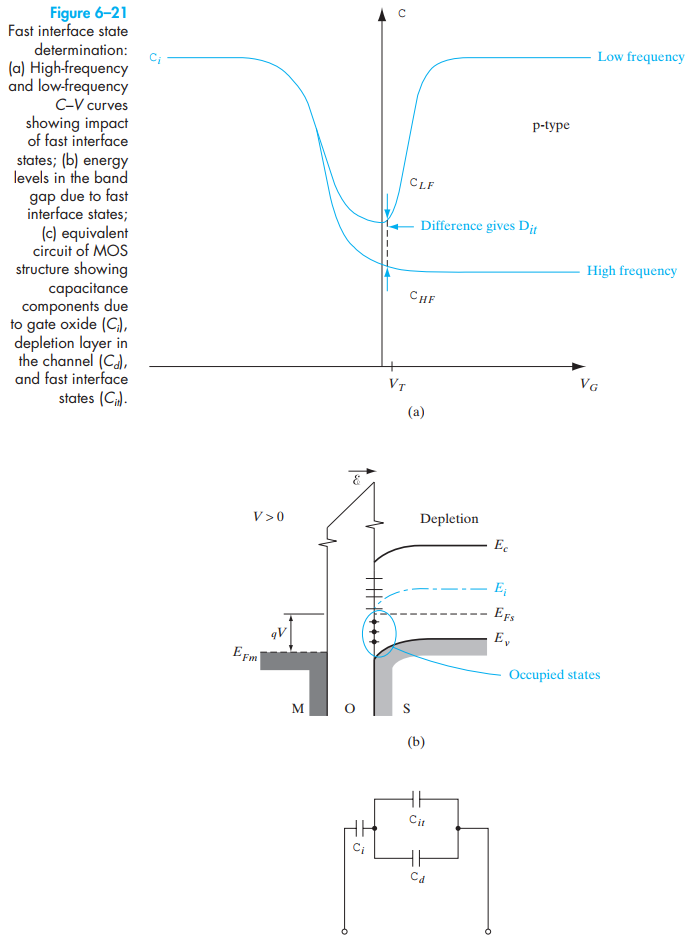
\includegraphics[width=0.7\textwidth]{fig6-21} \\ \hl \\~\\
		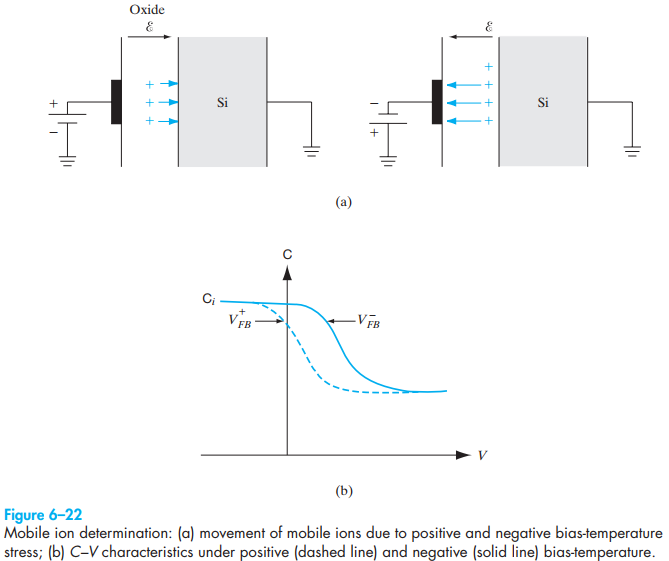
\includegraphics[width=0.7\textwidth]{fig6-22} \\ \hl \\~\\
		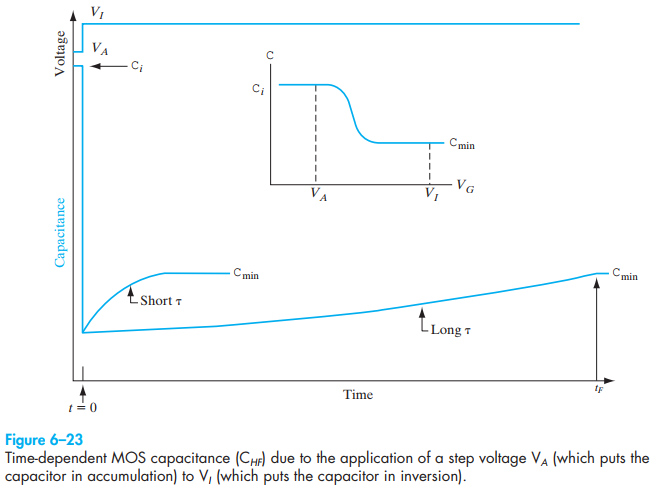
\includegraphics[width=0.7\textwidth]{fig6-23} \\ \hl \\~\\
		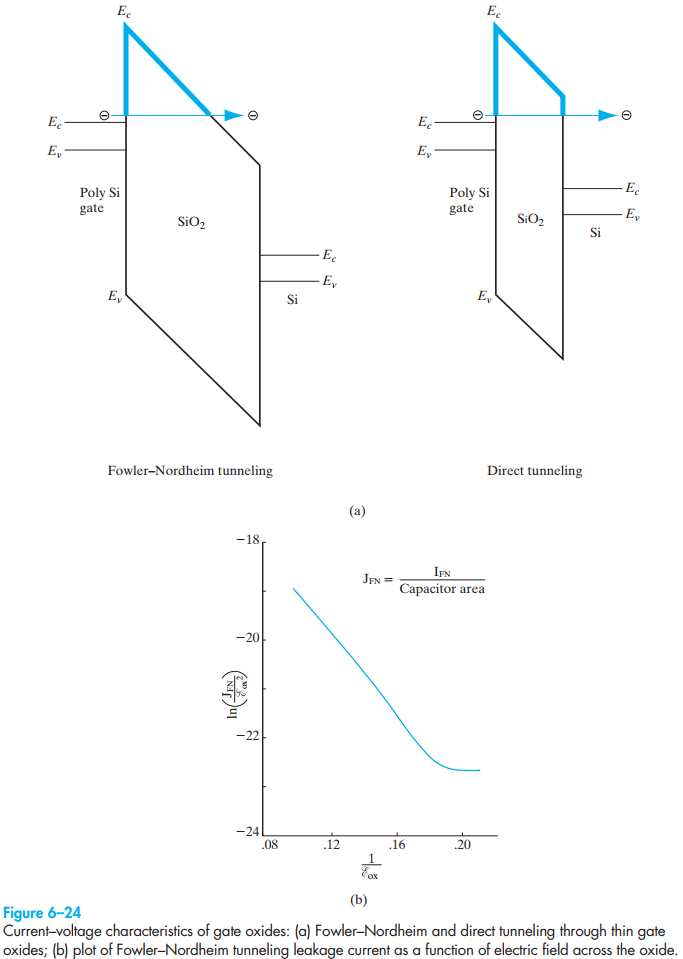
\includegraphics[width=0.7\textwidth]{fig6-24} \\ \hl \\~\\
		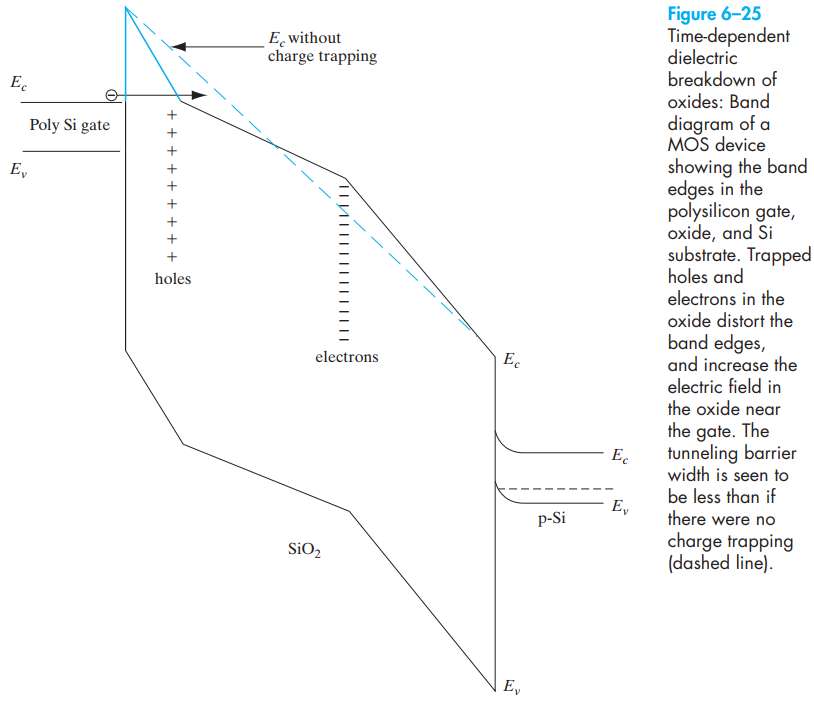
\includegraphics[width=0.7\textwidth]{fig6-25} \\ \hl \\~\\
		\sect{\Large{The MOS Field-Effect Transistor}}
		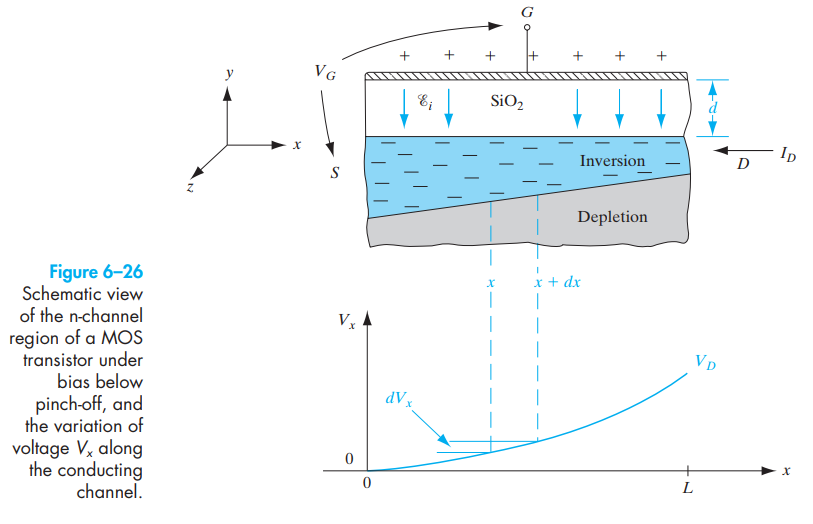
\includegraphics[width=0.7\textwidth]{fig6-26} \\ \hl \\~\\
		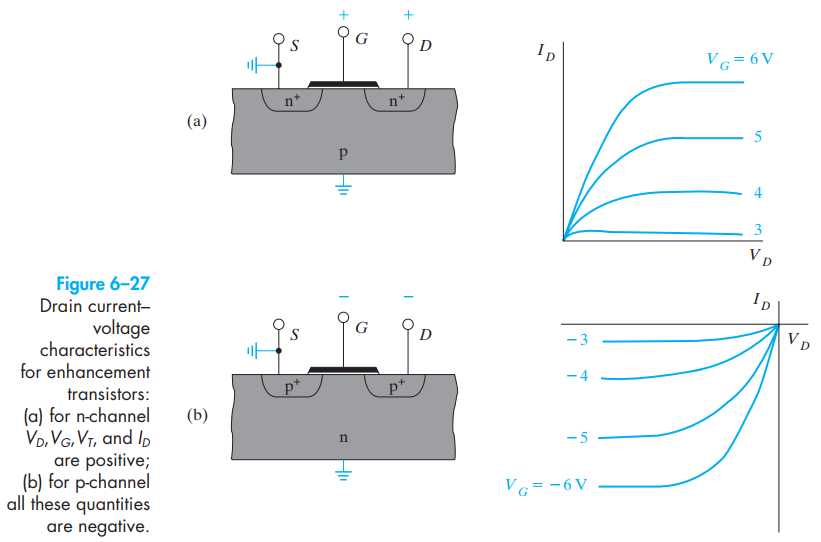
\includegraphics[width=0.7\textwidth]{fig6-27} \\ \hl \\~\\
		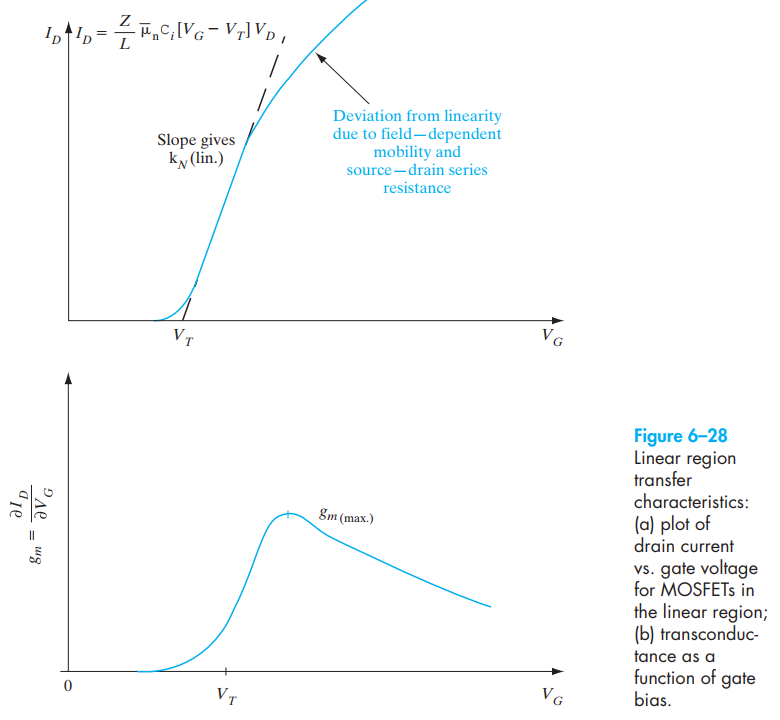
\includegraphics[width=0.7\textwidth]{fig6-28} \\ \hl \\~\\
		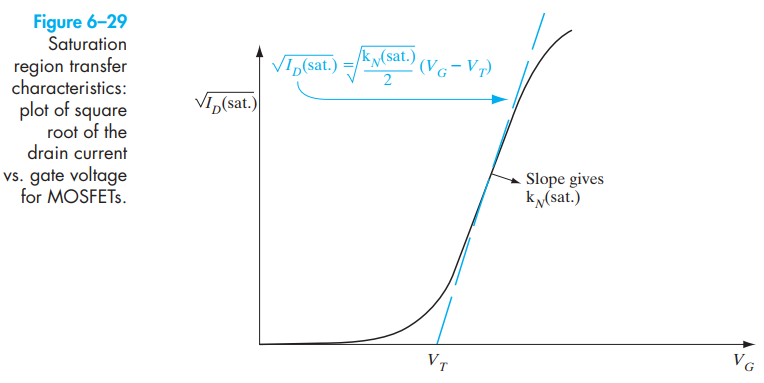
\includegraphics[width=0.7\textwidth]{fig6-29} \\ \hl \\~\\
		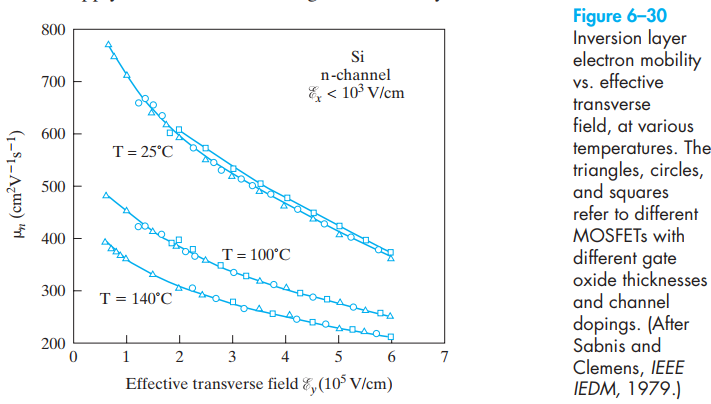
\includegraphics[width=0.7\textwidth]{fig6-30} \\ \hl \\~\\
		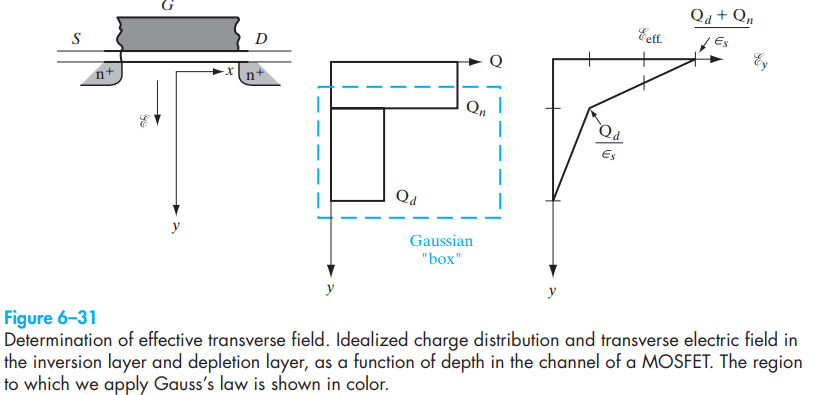
\includegraphics[width=0.7\textwidth]{fig6-31} \\ \hl \\~\\
		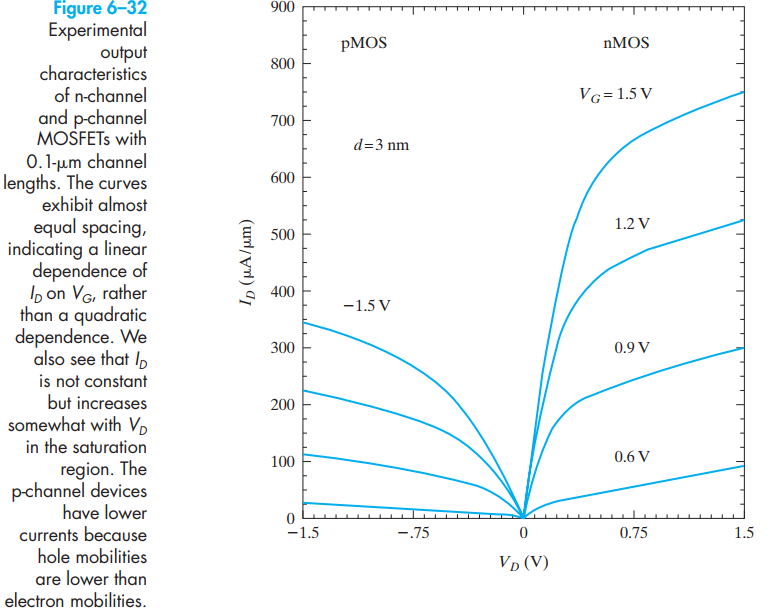
\includegraphics[width=0.7\textwidth]{fig6-32} \\ \hl \\~\\
		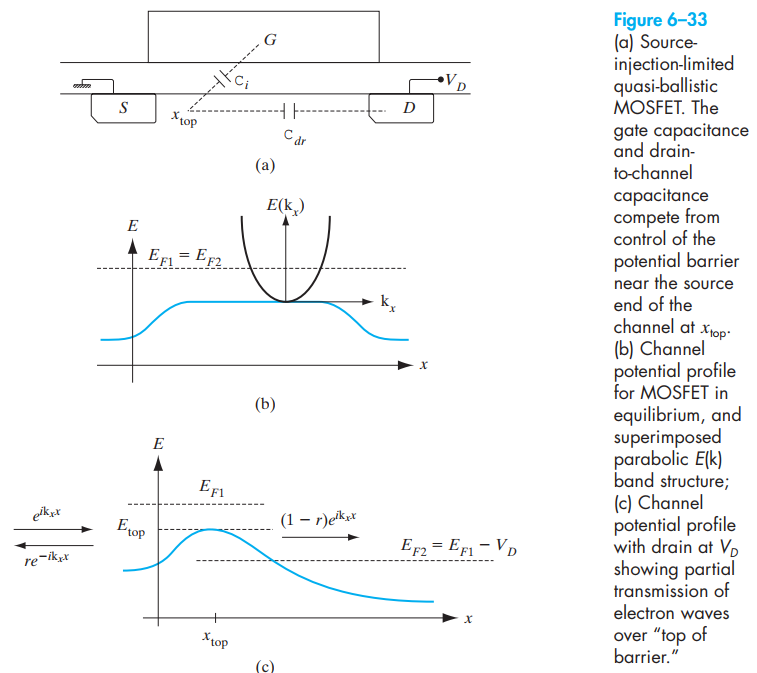
\includegraphics[width=0.7\textwidth]{fig6-33} \\ \hl \\~\\
		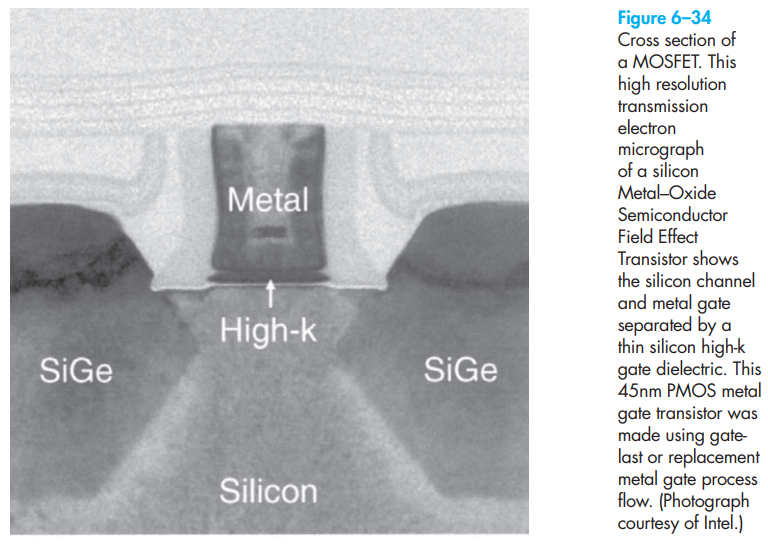
\includegraphics[width=0.7\textwidth]{fig6-34} \\ \hl \\~\\
		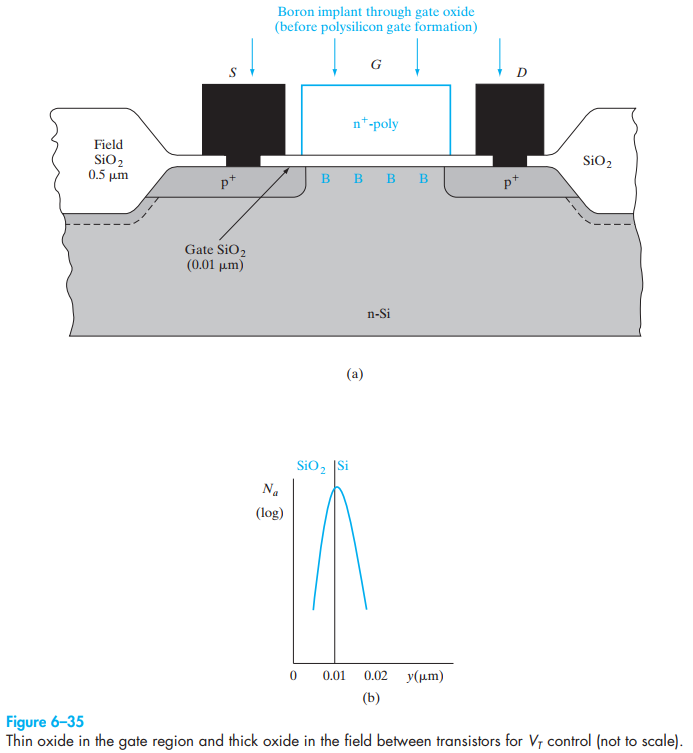
\includegraphics[width=0.7\textwidth]{fig6-35} \\ \hl \\~\\
		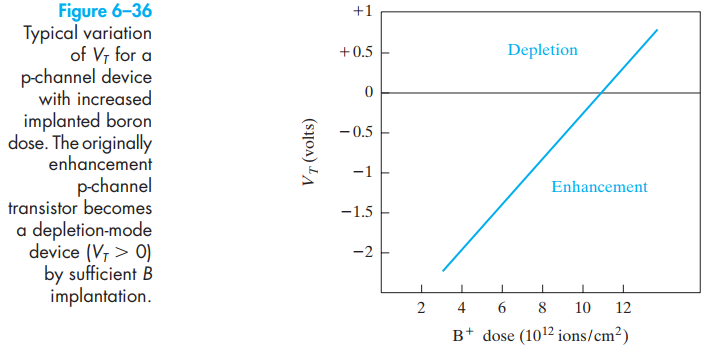
\includegraphics[width=0.7\textwidth]{fig6-36} \\ \hl \\~\\
		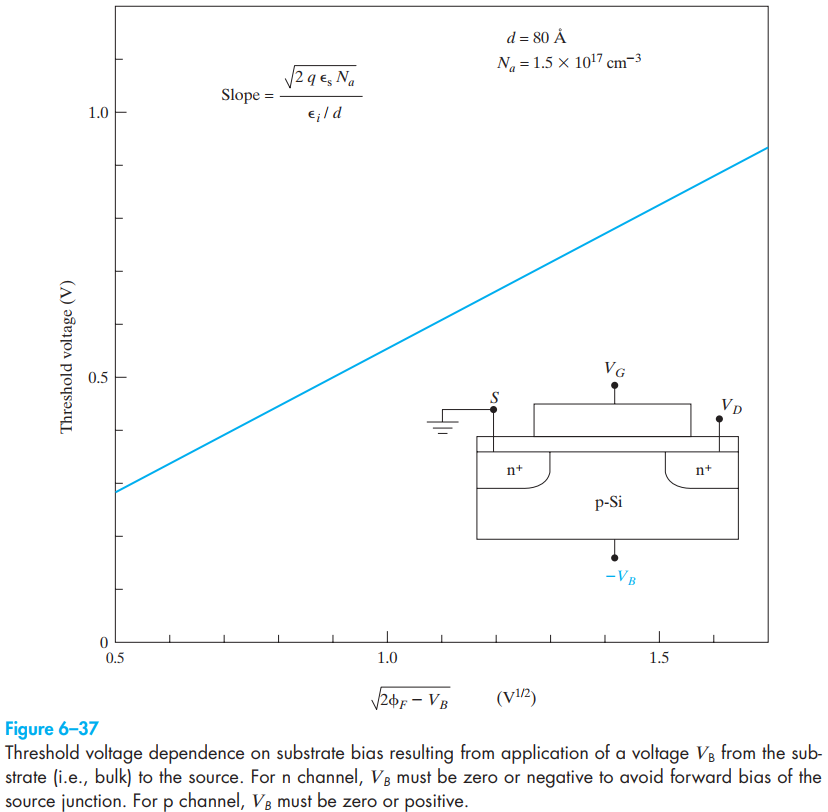
\includegraphics[width=0.7\textwidth]{fig6-37} \\ \hl \\~\\
		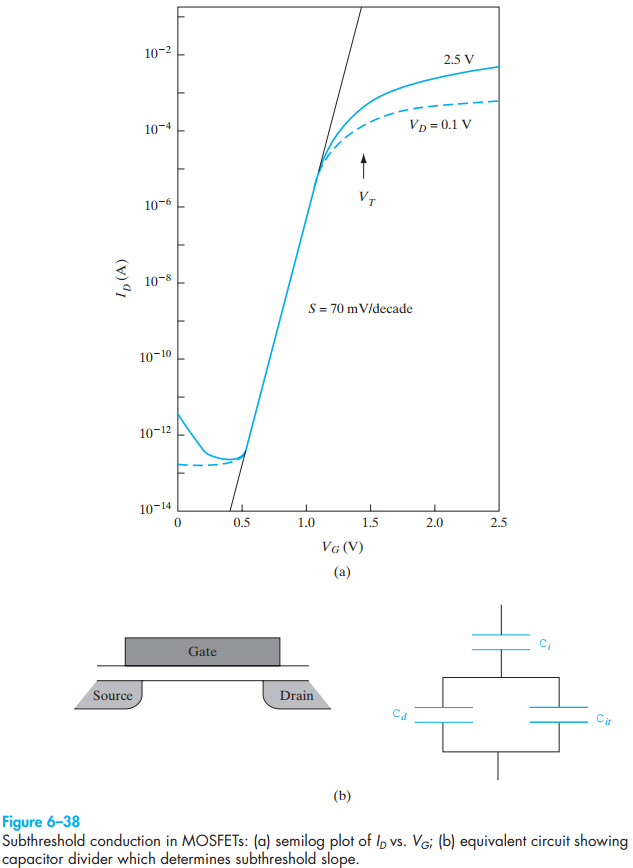
\includegraphics[width=0.7\textwidth]{fig6-38} \\ \hl \\~\\
		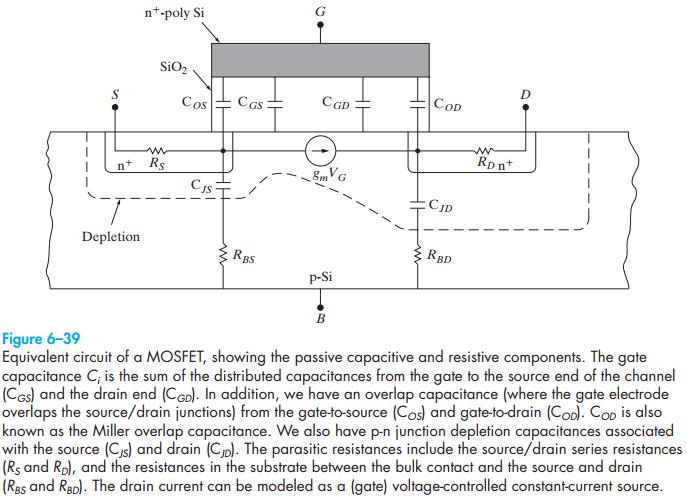
\includegraphics[width=0.7\textwidth]{fig6-39} \\ \hl \\~\\
		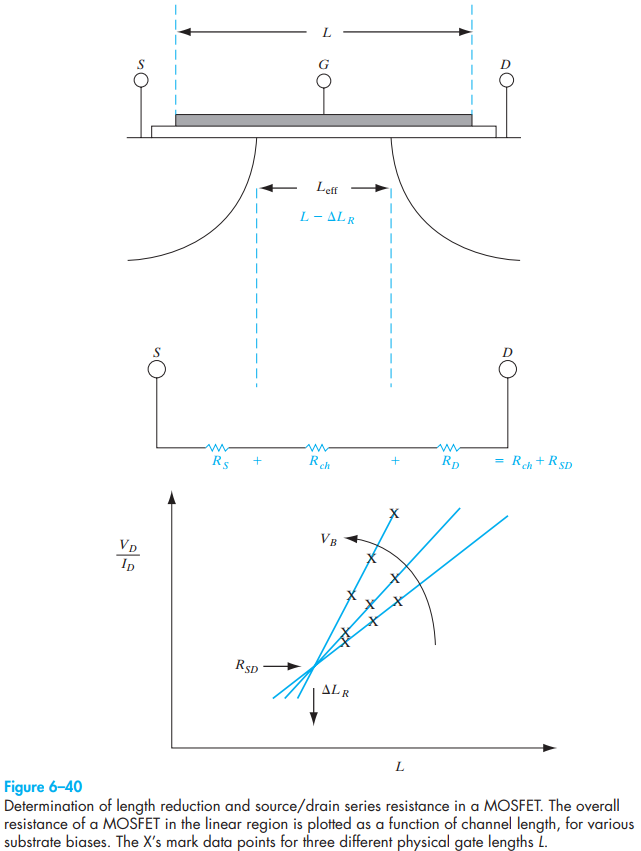
\includegraphics[width=0.7\textwidth]{fig6-40} \\ \hl \\~\\
		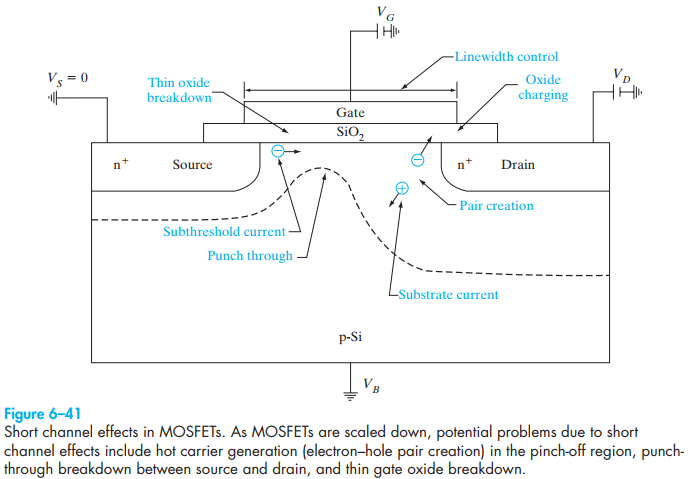
\includegraphics[width=0.7\textwidth]{fig6-41} \\ \hl \\~\\
		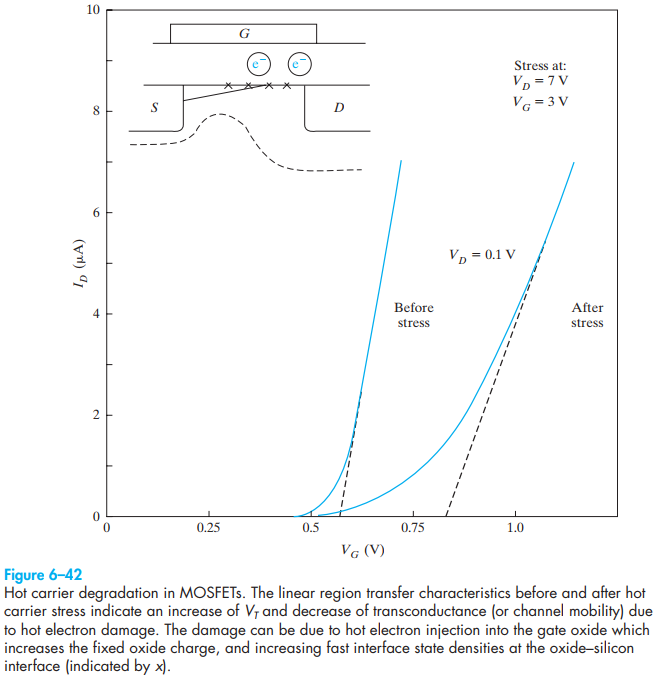
\includegraphics[width=0.7\textwidth]{fig6-42} \\ \hl \\~\\
		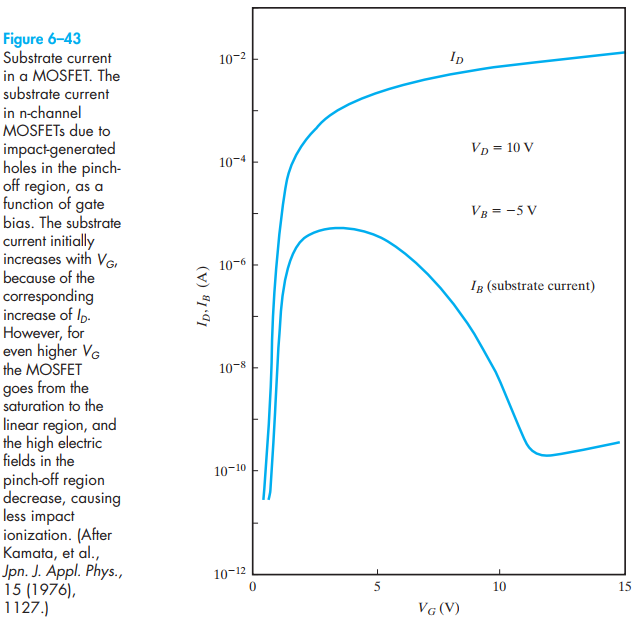
\includegraphics[width=0.7\textwidth]{fig6-43} \\ \hl \\~\\
		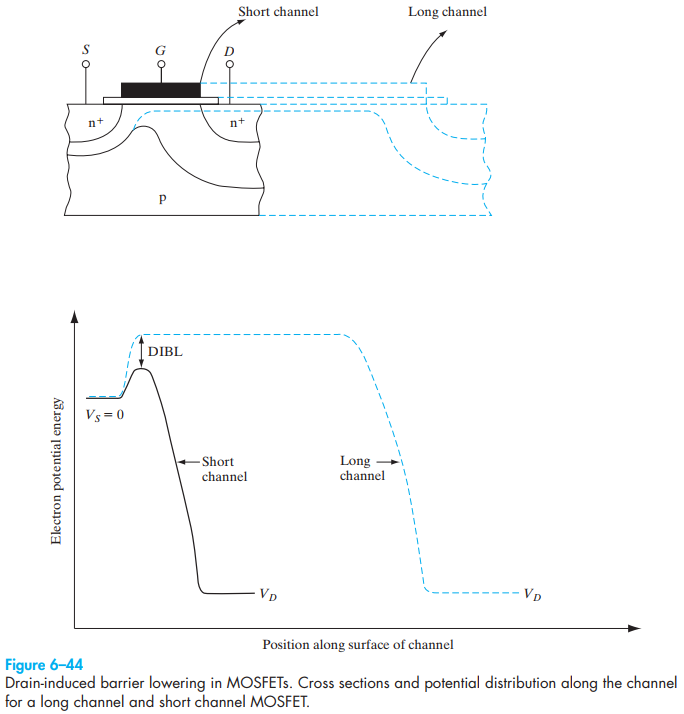
\includegraphics[width=0.7\textwidth]{fig6-44} \\ \hl \\~\\
		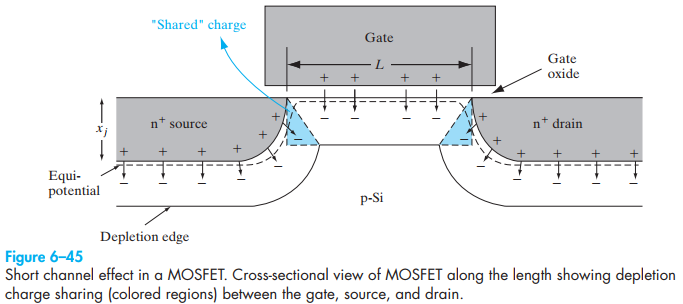
\includegraphics[width=0.7\textwidth]{fig6-45} \\ \hl \\~\\
		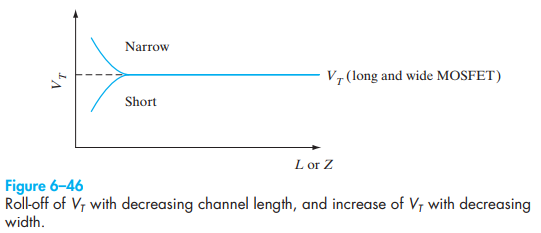
\includegraphics[width=0.7\textwidth]{fig6-46} \\ \hl \\~\\
		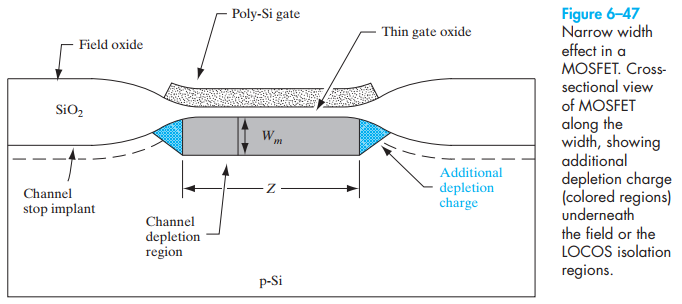
\includegraphics[width=0.7\textwidth]{fig6-47} \\ \hl \\~\\
		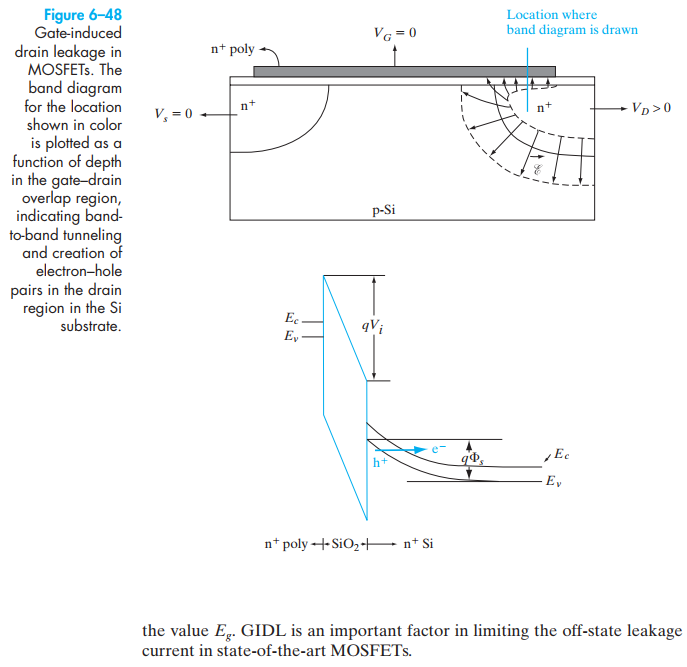
\includegraphics[width=0.7\textwidth]{fig6-48} \\ \hl \\~\\
		\sect{\Large{Advanced MOSFET Structures}}
		\includegraphics[width=0.7\textwidth]{fig6-49} \\ \hl \\~\\
		\includegraphics[width=0.7\textwidth]{fig6-50} \\ \hl \\~\\
	\end{center}
\end{document}